\documentclass[12pt]{jarticle} % Japanese
%\documentclass[12pt]{article} % English
% if there are problems in the above regarding fonts, use this
% \documentclass[UTF8]{ctexart}



%package
\usepackage{amsmath, newtxmath}
\usepackage[utf8]{inputenc}
%\usepackage{utf}
\usepackage{naist-jmthesis} %Japanese
%\usepackage{naist-mthesis} %English
\usepackage[dvipdfmx]{graphicx}
\usepackage[dvipdfmx]{hyperref}
\usepackage{pxjahyper} %Required pxjahyper.sty
\usepackage[dvipdfmx]{xcolor}
\usepackage{pxjahyper} %TOC文字化け対策



%definition
\definecolor{purple}{RGB}{98, 114, 164}
\hypersetup{
 colorlinks=true,
 linkcolor=black,
 citecolor=purple,
 urlcolor=black,
 pdfborder={0, 0, 1},
 linktoc=all
}



% Page style
\pagestyle{final}       % Camera-Ready
%\pagestyle{draft}      % Draft
\lang{Japanese} % Japanese
%\lang{English} % English
% Student Number
\studentnumber{1811147}
\doctitle{\mastersthesis}       % 修士論文
\major{\engineering}    % 工学



% 日本語題目 (in LaTeX)
%\title{再帰問い合わせ名前解決へのハッシュ関数を用いたDNS Exfiltration緩和策の提案}
\title{DNS Exfiltration対策を目的としたスーパーノード型P2Pネットワークに基づく名前解決システムの提案}
% 日本語題目 (in plain text)
%   注: (in LaTeX)と同じ場合は指定する必要なし。
%       この情報は修士論文/課題研究には現れませんが、管理のために必要です。
%\ptitle{再帰問い合わせ名前解決へのハッシュ関数を用いたDNS Exfiltration緩和策の提案}



% 英語題目 (in LaTeX)
%\etitle{Proposal for Mitigation of DNS Exfiltraion using Hash Function to Recursive Name Resolution}
\etitle{Proposal for Name Resolution System based on Supernode in P2P Networks against DNS Exfiltration}
% 英語題目 (in plain text)
%   注: (in LaTeX)と同じ場合は指定する必要なし。
%       この情報は修士論文/課題研究には現れませんが、管理のために必要です。
%\eptitle{Theoretical Studies on Low-Speed Calculation Algorithms of pi \\
%Utilizing the Sun and the Moon}
%\eptitle{Proposal for Mitigation of DNS Exfiltraion using Hash Function to Recursive Name Resolution}



% 日本語氏名 (in LaTeX)
%   (姓と名の間に空白を入れて下さい)
\author{高須賀 昌烈}
%\pauthor{}
%   (first name, last name の順に記入し、先頭文字のみを大文字にする。)
\eauthor{Shoretsu Takasuka}
% 別の例: \eauthor{Kurt G\"{o}del}
%\epauthor{}



% 論文提出年月日
\syear{2020}
\smonth{3}
\sday{15}



% 専攻の選択
%\department{\infproc}  % 情報処理学
%\department{\infsys}    % 情報システム学
%\department{\bioinf}   % 情報生命科学
\department{\infsci}    % 情報科学



% 審査委員(日本語)
%   (姓と名、名と称号の間に空白を入れて下さい)
%5人以上の場合,5人目以降は\addcmembers を使って宣言する。
%最大で合わせて8人まで宣言可能。
%主指導教員、副指導教員を明記する。両指導教員以外は委員。
%学外審査委員は、大学名を明記する
% 4人の場合
\cmembers{門林 雄基 教授}{(主指導教員)}
         {笠原 正治 教授}{(副指導教員)}
         {林 優一 教授}{(副指導教員)}
         {妙中 雄三 准教授}{(副指導教員)}
% 3人の場合
%\cmembers{○○ ○○ 教授}{(主指導教員)}
%         {○○ ○○ 教授}{(副指導教員)}
%         {○○ ○○ 准教授}{(副指導教員)}
%         {}{}
% 2人の場合
%\cmembers{○○ ○○ 教授}{(主指導教員)}
%         {○○ ○○ 教授}{(副指導教員)}
%          {}{}
%          {}{}



% 審査委員(英語)
%     (first name, last name の順に記入し、先頭文字のみを大文字にする。
%       first name と last name の間に空白、
%       last name と 称号の間にカンマと空白を入れて下さい。)
% 5人以上の場合,5人目以降は\eaddcmembers を使って宣言する
% Supervisor, Co-supervisor, and Member must be specified.
% 4人の場合
\ecmembers{Professor Youki Kadobayashi}{(Supervisor)}
          {Professor Shoji Kasahara}{(Co-supervisor)}
          {Professor Yu-ichi Hayashi}{(Co-supervisor)}
          {Associate Professor Yuzo Taenaka}{(Co-supervisor)}
% 3人の場合
%\ecmembers{Professor xx xx}{(Supervisor)}
%          {Professor xx xx}{(Co-supervisor)}
%          {Associate Professor xx xx}{(Co-supervisor)}
%          {}{}
% 2人の場合
% \ecmembers{Professor xx xx}{(Supervisor)}
%           {Professor xx xx}{(Co-supervisor)}
%           {}{}
%           {}{}
% キーワード5〜6個 (in LaTeX)
%\keywords{$\pi$, 天文学, 数学, 計算機, アルゴリズム}



% ===================キーワード===================
\keywords{ネットワークセキュリティ,ドメインネームシステム,秘匿通信,分散ハッシュテーブル,スーパーノード型ピアツーピア}
% キーワード5〜6個 (in plain text)
%   注: (in LaTeX)と同じ場合は記入する必要なし。
%       この情報は修士論文/課題研究には現れませんが、管理のために必要です。
%\pkeywords{pi, 天文学, 数学, 計算機, アルゴリズム}
%\pkeywords{DNS Exfiltration, 秘匿通信,ハッシュ関数,再帰問い合わせ}
% 5 or 6 Keywords (in LaTeX)
%\ekeywords{$\pi$, astronomy, mathematics, computer, algorithm}



% ===================Keyword===================
\ekeywords{Network Security, Domain Name System(DNS), Covert Channel, Distributed Hash Table(DHT), Supernode in Peer-to-Peer}
% 5 or 6 Keywords (in plain text)
%   注: (in LaTeX)と同じ場合は記入する必要なし。
%       この情報は修士論文/課題研究には現れませんが、管理のために必要です。
%\epkeywords{pi, astronomy, mathematics, computer, algorithm}
%\epkeywords{DNS Exfiltration, Covert Channel, Hash Function, Recursive Name Resolution}



% ===================内容梗概===================
\abstract{
}
%   注: 行の先頭が\\で始まらないようにすること。
%   注: (in LaTeX)と同じ場合は記入する必要なし。
%       この情報は修士論文/課題研究には現れませんが、管理のために必要です。
%       改行する箇所には空白行を入れる。
%       行の先頭が\\で始まらないようにすること。
%\pabstract{
%}
% Abstract (in LaTeX)
%  注:  行の先頭が\\で始まらないようにすること。



% ===================Abstruct===================
\eabstract{
}
% Abstract (in plain text)
%   注: (in LaTeX)と同じ場合は記入する必要なし。
%       この情報は修士論文/課題研究には現れませんが、管理のために必要です。
%       改行する箇所には空白行を入れる。
%       行の先頭が\\で始まらないようにすること。
%\epabstract{
%The calculation of pi has been paid much attention since human beings
%appeared on the earth.
%This thesis presents novel low-speed algorithms to calculate
%pi utilizing the sun and the moon.
%This is a sample abstract. This is a sample abstract.
%}



% ===================表紙===================
\begin{document}
\titlepage
\cmemberspage
\firstabstract
\secondabstract



% ===================目次===================
\toc
\newpage
\listoffigures
%\newpage
\listoftables



% ===================本文===================
\newpage
\pagenumbering{arabic}
\section{序論}
\subsection{背景}
ドメインネームシステム(Domain Name System, DNS)は,ドメイン名(E.g. www.example.com)をインターネット上でのノードの住所を表すIPアドレス(E.g. 93.184.216.34)に変換する機能を担っており,DNSを通じて特定した宛先に問い合わせることで我々はサービスにアクセスできている.
現在のインターネットの利活用において,名前解決の仕組みは極めて重要な技術の一つである.
しかし,性善説的な当時の設計に伴い生じた脆弱性を利用した攻撃がいくつか報告されている.
1987年にRFC1034, RFC1035(\cite{rfc1034, rfc1035})として公開されたDNSのコンセプトは,現在もなお本質的な仕組みは変更されることなく適用されている.
%近年では,平文であるDNSクエリを解析することでユーザがどのwebページを閲覧しようとしているのか,どこにメールを送信しようとしているのかといったユーザのプライバシーを侵害される脅威\cite{rfc7626}に関心が集まっており,HTTPSやTLSによってクエリおよび応答パケットを暗号化するDoH/DoTが盛んに議論されている.
その設計に起因する課題の内,DNSクエリのラベルおよびリソースレコード(Resource Record, RR)をデータ転送のメディアとするDNS Tunnelingがある.

DNS Tunnelingは,一般にフィルタリングされることが少ないDNSの特徴とDNSがデータ転送のメディアとして機能しているとは想像しない人の認知の隙間をついた手法であり,ファイヤー・ウォールやIDS/IPSといったセキュリティラインを突破するために使用される.
このように本来の目的とは違う方法でデータを転送する手法は,一般に秘匿通信(Covert Channel)と呼ばれる\cite{covertchannel}.
DNS Tunnelingは,秘匿通信の代表例であり,マルウェアとC2(Command \& Control)サーバとの通信の秘匿手法,または,ターゲットから取得したデータを外部に流出させるといった目的実行の手段として,実際のインシデントで広く利用されている\cite{frameworkpos, bondupdater, bernhardpos, multigrainpos, pisloader, denis, dnsmessenger, udpos}.
%2014年には,発生した大規模なクレジットカード情報流出事件\cite{},最近では2019年に発生したAPTグループ(通称,OilRig)による中東政府を標的とするサイバー攻撃のC2通信\cite{bondupdater}として実際のインシデントなどがある.
%このDNS Tunnelingのメカニズムは,スタブリゾルバからリカーシブサーバを経由し権威サーバへ問い合わせる一連の正規の仕組みに基づいており,名前解決を実現するにあたり生じる設計上の脆弱性を突いた手法である.
従来のDNS Tunnnlingに対するアプローチには,検知による手法が採用されてきた.
DNS TunnelingによるDNSクエリは,以下(\ref{eq:sample_qname})に示すように,転送量に比例して長いラベルを持ち,ラベルとしての文字列制約を満たすためのエンコーディングによって高いエントロピーを示す特徴がある.

\begin{eqnarray}
 \label{eq:sample_qname}
 \begin{aligned}
  &obqxg43xmqytcmjr.exfil.com\\
  &base32(password1111) = obqxg43xmqytcmjr
 \end{aligned}
\end{eqnarray}

また,インタラクティブなシェルなど双方向の通信をDNS Tunnelingで実現しようとする場合,時間あたりに高頻度なトラフィックが発生するという特徴が現れる.
このような特徴に基づき,パターンマッチングや機械学習,文字列分布などのメソッドを用いた検知手法が過去に多数考案されてきた\cite{born, cheng, liu, asaf, steadman, jawad}.
それら検知手法は,かなり高い精度で分類を実現しているものがあるが,DNS Tunnelingとして検知する対象としているパケットには一般に利用することができるDNS Tunnelingツールキット\cite{ozymandns, iodine, dnscat2}が使用され,それらは特に過剰な特徴量を示し,明らかに正規のDNSクエリと異なる特徴がある.
高い精度を示す従来の検知手法だが,しかし,それらを迂回する手法として,1回あたりの転送データ量を少なくすることで特徴量を減らすLow Throughputなバイパス手法,また,パケット間のインターバルを数日・数ヶ月と長期化させることでファイル肥大から一定期間しか保存されることがないログ管理の隙間を突いたSlowなTunenling手法があり,従来の検知手法では対応することが困難である.
悪意を持つユーザの視点として,1bitでも転送できることは秘匿通信として利用することができるため,転送量の少なさは軽視されるべきではない.

他方で,DNSは初めに述べたように,現在のインターネットの根幹技術として根ざしており,抜本的な改変は期待されない.
すなわち,既存のDNSによる名前解決のメカニズムに大幅な改変を加えないという制約下で,Tunnelingに対処することが現実的な最適解であると考える.


\subsection{目的}
本研究では,既存のDNSの名前解決メカニズムの大部分を流用することが一部の改変に留めながら,DNSを用いたデータ転送としての機能の排除を実現する次世代の名前解決メカニズムを提案する.
%\subsection{貢献点}
%本研究の貢献は,以下の通りである.
%\begin{itemize}
% \item 侵入通信を目的とするDNS Tunnelingに対するリアルタイム検知アルゴリズムの提案
% \item 既存対策アプローチとDNSの潜在的データ転送脅威モデルの検討
%\end{itemize}
%\subsubsection{脅威モデル}
%\subsubsection{仮説}




\subsection{本論構成}
%\ref{kako}節では、過去における研究について述べ、
%\ref{kadai}章では、現状と今後の課題について述べる。
%また、付録\ref{omake1}におまけその1を添付する。
本稿の構成は以下の通りである.
まず第2章で,準備として,DNSプロトコル・秘匿通信・Tunnelingメカニズム・分散データベースの4点について説明する.
第3章では,関連研究としてトラフィックおよびペイロード特徴に基づいた検知手法を説明し,それら手法がLow Throughput手法・Slow Tunneling手法に対して検知が困難であることを説明する.
第4章で提案手法とその実装について述べ,第5章で提案手法の性能評価と考察行い,第6章で残留する脅威モデルについて議論する.
最後に,第7章で結論と今後の課題について述べていく構成になっている.



\newpage
\section{準備}
本章は第3章以降の要素補足を目的に,本論において核となる技術内容・特徴およびそのメカニズムについて説明する.
\subsection{DNS プロトコル概要}
\label{sec:dns-protocol}
DNS(Domain Name System)は,インターネットに接続された無数のコンピュータを一意に識別するためのIPアドレスを,人が認識しやすいドメイン名に変換するシステムである.
元来,インターネット上でのホストの識別にはIPアドレスが使用されてきた.
しかし,32bitの名前空間で10進数表記のIPv4(E.g. ``192.168.0.1"),もしくは,128bitの名前空間で16進数表記のIPv6(E.g. ``2001:200:16a:8::230")は,人にとって認識しにくいものである.
そのため,自然言語のようにアルファベットや数字で表記する方法が取られ,当初はその対応表であるhosts.txtが中央集権的に管理されていたが,やがてホスト数の増大に伴い管理が困難になっていき,提案されたのが対応表を分散的に管理するDNSである.

DNSのシステムアーキテクチャは,クライアント・サーバ構成で成り立っている.
一般に,クライアントがドメインを問い合わせた場合,サーバはドメインに対応づけているIPアドレスを応答することで,クライアントはドメインに対応づけられたIPアドレスを解決することができる.
ドメインからIPアドレスの解決は正引きと呼ばれ,IPアドレスからドメインの解決を逆引きと呼ぶ.

ドメインは,数字とアルファベットおよびハイフン(``-")の文字列で表記され,最大長は63オクテットと定義されている.
また,ドメインはルートを頂点とする階層構造をとり,各階層にはドメインを管理する主体が存在し,管理主体を委譲することによって分散的にデータベースを管理する仕組みを取っている.

\begin{figure}[h]
 \centering
 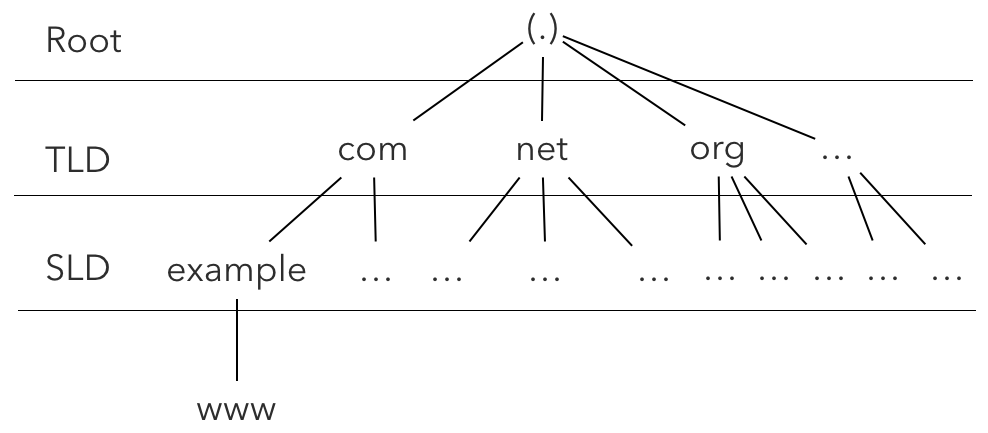
\includegraphics[width=12.0cm]{images/dns-architecture.png}
 \caption{ドメインにおける名前空間}
 \label{dns-exfiltration}
\end{figure}

ドメイン名は,ドメインに相当するラベルをドット区切りで表され,最大長は255オクテットである.
ドメイン名は右から順に階層序列が表現され,ドットで表現されるルートは一般には省略される.
最も右に位置づくラベルがTLD(Top Level Domain)であり,そのTLDからn番目(n $\mid$ n $\in$ $\mathbb{N}$)のラベルが第 n レベルドメインである.

TLDを大別すると,``.com"や``.net"をはじめとした特定分野別のgTLD(global Top Level Domain),``.jp"や``.ch"のような国ごとに割り当てられているccTLD(Co\\untry Code Top Level Domain)の二つに分けられる.
%TLDごとに登録するプロセスや必要書類,金額は異なり,上いの

\subsubsection{ノードの種類}
DNSは,機能に応じて3つに分類することができる.

\subsubsection{リソースレコード}
DNSの仕組みにおいて,ドメイン名に関連づけられた情報は,IPアドレス以外にも様々なものがあり,それらはリソースレコード(Resorce Record, RR)と呼ばれる.
DNSの仕組みによって,権威サーバが提供できる情報はドメイン名とIPアドレスの対応情報だけではない.
最も一般的なレコードは,Aレコードであり,FQDNをIPv4アドレスにマッピングする.
権威は,サブドメインへ委譲することが可能である.この機能は,NSレコードによって実現される.

\subsection{DNS Tunneling}
\label{sec:dns-tunnel}
DNSを利用して情報を外部に転送するには,初めにデータの宛先となるドメイン(E.g. exfil.com)を作成することになる.
転送する際のキャリアとなるDNSクエリのラベルには,使用できる文字列は数字・アルファベット・ハイフン(``-")である必要があるため,一般にBase32・64を用いて転送したい情報をエンコーディングすることでこの制約条件を満たす.
用意できたQNAME(E.g. arbitrary-string.exfil.com)について,例えばAのリソースレコードをクエリすると,サブドメインの存在の有無に関わらず,宛先となるドメイン(exfil.com)に任意の情報を転送することができるという具合である.
以下\ref{fig:dns-exfiltration}に,DNS Exfiltrationのメカニズムについて図解する.

\begin{figure}[h]
 \centering
 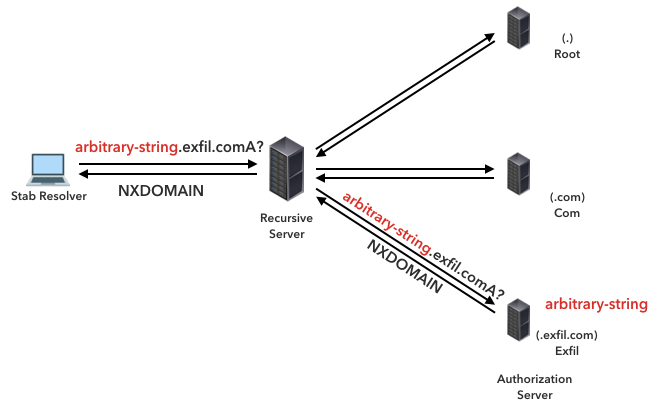
\includegraphics[width=12.0cm]{images/dns-exfiltration.png}
 \caption{arbitrary-stringという任意の文字列が,DNSクエリのラベル部を用いて,事前に用意した権威サーバ(exfil.com)に転送される様子.}
 \label{fig:dns-exfiltration}
\end{figure}

また,管理する権威サーバのドメインに適当なホスト名(E.g. www)を作成し,そのホスト名のリソースレコード(E.g. TXT)に情報を付与していた場合には,そのホストへの問い合わせを通じて逆方向,すなわち権威サーバから任意の情報を転送することができる.
DNSのリソースレコードを転送キャリアとする流入通信のメカニズムを図解した様子が,\ref{fig:dns-tunneling}である.

\begin{figure}[h]
 \centering
 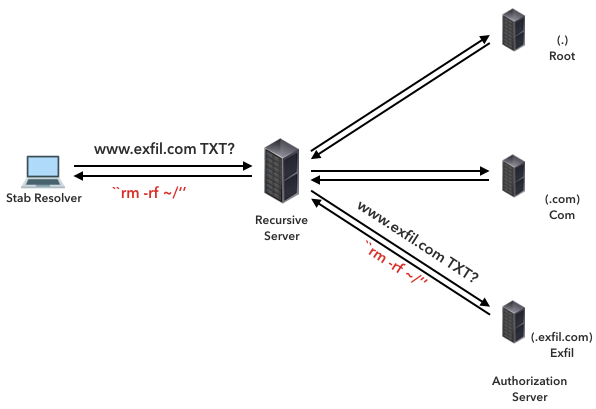
\includegraphics[width=10.0cm]{images/dns-tunneling.png}
 \caption{事前にTXTレコードに登録された情報を問い合わせることで,権威サーバからの命令情報を取得している様子.}
 \label{fig:dns-tunneling}
\end{figure}

このようなDNSを用いて双方向な通信手法がDNS Tunnelingである.
%1998年4月,DNS Tunnelingの手法は,NmapのBugtraqメーリングリストにて初めて公になったとされている\cite{bugtraq}.


%\subsubsection{DNS Tunneling 特徴}
%%\subsubsection{その他課題}
%%\subsection{秘匿通信}
%%秘匿通信(英Covert Channel)とは,
%%情報転送を実現するにあたり,データの転送を本来の設計としていないプロトコルにそのデータを注入する手法である.
%%\subsubsection{ステガノグラフィ}
%%\subsubsection{代替プロトコル}
%\subsection{分散ハッシュテーブル}
%\subsubsection{アルゴリズム}
%\subsubsection{暗号学的ハッシュ関数}
%\subsection{P2P}
%\subsubsection{アーキテクチャ}



\newpage
\section{関連研究}
\label{sec:related-works}
本章では,はじめに既存のDNS Tunnelingに対するアプローチとして提案されている検知アプローチを取り上げ,現在の検知に基づく対策の課題として,Low Throughput手法とSlowな転送手法というバイパス手法に対処できないことを明らかにする.
次に,これまでに提案されてきたP2Pベースの名前解決システムを説明し,提案手法との違いを示す.
%また,新しいアーキテクチャを導入するとき 既存のシステムとのマイグレーションを考慮する必要がある点について,本提案手法がマイグレーションを考慮している設計である点について
%最後に,既存の検知手法および次世代名前解決システムの課題から,既存のシステムに迎合しながらDNS Tunnelingを緩和する名前解決システムの必要性を明らかにする.

\subsection{検知に基づくDNS Tunneling対策手法}
%\subsubsection{パターンマッチング}
%\subsubsection{同一ドメインあたりのクエリ頻度}
%\subsubsection{Qnameにおける文字列分布}
%\subsubsection{Qnameにおける長さとエントロピー}
%\subsubsection{課題 : Low ThroughputなTunnelingに対する検知手法}
DNS Tunnelingメソッドを使用した時のDNSクエリは,\ref{sec:dns-tunnel}で述べたような特徴が現れる性質がある.
これまで,DNS Tunnelingに対して,正規のDNSトラフィックと分類する手法は数多く提案されており,それら手法は大別すると統計ベース・機械学習ベース多クラス・機械学習ベースバイナリクラスに区別することができる.

%\subsection{悪性DNS検知に関する研究}
\subsection{P2Pベース名前解決システム}
%\subsubsection{Blockchainベース - Namecoin, Blockstack}
%\subsubsection{P2Pベース - GNS(Gnu Name System)}
これまでに,DNSにおける〜の課題に対して,P2Pに基づいた名前解決システムは数多く提案されてきた.

\subsection{既存研究のまとめ}



\newpage
\section{提案手法}
%\subsection{本研究の位置づけ}
%\subsection{脅威モデル}
\ref{sec:related-works}で述べたように,これまでに提案されてきたDNS Tunnelingに対する検知に基づく手法には,Low Throughput手法および転送頻度を下げる手法に対して,高い精度を実現するのが困難であるという課題がある.
他方,新しいアーキテクチャに基づく名前解決システムには,マイグレーションの課題が残留している.

本章では,上記内容を踏まえ,DNS Exfiltrationを防止する名前解決システムS-NRS(Supernode in P2P networks based Name Resolution System)について説明する.

\subsection{S-NRS}
\subsubsection{設計とアーキテクチャ}
S-NRSのアーキテクチャでは,役割に応じてノードは4つに大別することができる.
スタブリゾルバは既存のDNSと変更はなく,DNSクライアントとして,名前解決を依頼する主体として位置づくノードである.
リカーシブサーバは,スタブリゾルバからの問い合わせに対してリソース情報を保持する主体に代理的に問い合わせ機能と,問い合わせた情報を一定期間キャッシュするキャッシュサーバとして機能するノードである.
既存のDNSにおける権威サーバは,リカーシブサーバからの問い合わせに応答するマネージャと,リソース情報について作成・消去および更新などの操作をするプロバイダの二つに分けられる.
S-NRSにおいて,リソース情報は,オブジェクト(object)とリソースレコードタイプ(rtype)を引数とするハッシュ関数から算出されるコンテンツIDが紐づけられ,そのコンテンツIDに基づきハッシュ空間上に対応づけられる.
各マネージャは,ハッシュテーブル全体のうち連続した幾らかの管理範囲が割り当てられ,範囲下にあるコンテンツIDに基づいたリソース情報を保存・管理する.
このようにして,リソース情報は,特定の範囲ごとに分割されたハッシュテーブルにて分散的に管理される.
マネージャ同士は,フルメッシュなネットワーク構造で接続し合い,各マネージャには地理的・意味的類似なプロバイダが階層的な序列に基づき接続される.

プロバイダからリソース情報への操作リクエストがあった際には,リソース情報のコンテンツIDを算出し,そのIDが含まれるハッシュ空間を管理する担当マネージャに操作依頼を転送し,受け取った担当マネージャは直ちに,リソース情報への操作を実行する.


%\begin{figure}[h]
% \centering
% \includegraphics[width=10.0cm]{images/spnrs-architecture.png}
% \caption{SPNRSによって,名前解決している様子.}
% \label{fig:spnrs-architecture}
%\end{figure}


%\subsubsection{想定する脅威}
%\subsubsection{名前解決メカニズム}
\subsubsection{通信プロトコル}
%\subsubsection{KVSモデルに基づく分散ハッシュテーブル}
\subsection{課題}
%\subsubsection{QNAMEとRRを引数とするハッシュ値をキーとするクエリ}
%\subsection{データベース}


\newpage
\section{評価}
\subsection{DNS Exfiltrationに対する定性評価}
\subsection{シミュレーション実験に基づく定量評価}
\subsubsection{シミュレーション実験構成}
\subsubsection{肥大化したリクエストペイロードサイズ}
\subsubsection{RTT(Round Trip Time)}
\subsubsection{トラフィック量}

\newpage
\section{議論}
\subsection{最適なハッシュ計算ノード}
\subsection{流入通信に対するリソースレコード}
%\subsubsection{CNAME, MX}
%\subsubsection{DNSKEY - 公開鍵検証}
%\subsubsection{TXT - ドメイン検証}

\newpage
\section{結論}
\subsection{まとめ}
\subsection{今後の課題}


% ===================謝辞===================
\newpage
\acknowledgements
ご指導ご鞭撻賜りありがとうございました.




% ===================参考文献===================
% ここでは \reference を使って、自分でリストを作るか、BibTeX を使って
% リストをつくって下さい。この例では BibTeX を作るような形式になってい
% ます。
\newpage
%\reference
%\bibliographystyle{plain}
\begin{thebibliography} {25}\small
 \bibitem{rfc1034} P.V. Mockapetris. ``Domain names - concepts and facilities. RFC 1034 (INTERNET STANDARD)," November 1987. Updated by RFCs 1101, 1183, 1348, 1876, 1982, 2065, 2181, 2308, 2535, 4033, 4034, 4035, 4343, 4035, 4592, 5936.
 \bibitem{rfc1035} P.V. Mockapetris. ``Domain names - implementation and specification. RFC 1035 (INTERNET STANDARD)," November 1987. Updated by RFCs 1101, 1183, 1348, 1876, 1982, 1995, 1996, 2065, 2136, 2181, 2137, 2308, 2535, 2673, 2845, 3425, 3658, 4033, 4034, 4035, 4343, 5936, 5966, 6604."
 \bibitem{covertchannel} ICANN, ``What Is an Internet Covert Channel?," August 2016. \href{https://www.icann.org/news/blog/what-is-an-internet-covert-channel}{https://www.icann\\.org/news/blog/what-is-an-internet-covert-channel}. (accessed 2019-12-12).
 \bibitem{rfc7626} S. Bortzmeyer. ``DNS Privacy Considerations RFC 7626 (INTERNET STANDARD), " August 2015.
 \bibitem{frameworkpos} KrebsonSecurity. ``Deconstructing the 2014 Sally Beauty Breach," May 2015. \href{https://krebsonsecurity.com/2015/05/deconstructing-the-2014-sally-beauty-breach/}{https://krebsonsecurity.com/2015/05/deconstructing-the-2014-sally-beauty-breach/}. (accessd 2019-11-30).
 \bibitem{bondupdater} IronNet. ``Chirp of the PoisonFrog," February 2019. \href{https://ironnet.com/blog/chirp-of-the-poisonfrog/}{https://ironnet.com/blog/ch\\irp-of-the-poisonfrog/}. (accessd 2019-11-30).
 \bibitem{bernhardpos} Nick Hoffman. ``BernhardPOS," July 2015. \href{https://securitykitten.github.io/2015/07/14/bernhardpos.html}{https://securitykitten.github.io/2015/\\07/14/bernhardpos.html}. (accessd 2019-11-30).
 \bibitem{multigrainpos} Fireeye. ``MULTIGRAIN – Point of Sale Attackers Make an Unhealthy Addition to the Pantry," April 2016. \href{https://www.fieeye.com/blog/threat-research/2016/04/multigrain\_pointo.html}{https://www.fieeye.com/blog/threat-research/2016/04/multigrain\_pointo.html}. (accessd 2019-11-30).
 \bibitem{pisloader} Palo alto Networks. ``New Wekby Attacks Use DNS Requests As Command and Control Mechanism," May 2016. \href{https://unit42.paloaltonetworks.com/unit42-new-wekby-attacks-use-dns-requests-as-command-and-control-mechanism/}{https://unit42.paloaltonetworks.com/unit42-new-wekby-attacks-use-dns-requests-as-command-and-control-mechanism/}. (accessd 2019-11-30).
 \bibitem{denis} Kaspersky. ``Use of DNS Tunneling for C\&C Communications," April 2017. \href{https://securelist.com/use-of-dns-tunneling-for-cc-communications/78203/}{https://securelist.com/use-of-dns-tunneling-for-cc-communications/78203/}. (accessd 2019-11-30).
 \bibitem{dnsmessenger} CISCO Talos. ``Spoofed SEC Emails Distribute Evolved DNSMessenger," October 2017. \href{https://blog.talosintelligence.com/2017/10/dnsmessenger-sec-campaign.html}{https://blog.talosintelligence.com/2017/10/dnsmessenger-sec-campaign.html}. (accessd 2019-11-30).
 \bibitem{udpos} Cylance. ``Threat Spotlight: Inside UDPoS Malware," Febrary 27 2018. \href{https://threatvector.cylance.com/en\_us/home/threat-spotlight-inside-udpos-malware.html}{https://threatvector.cylance.com/en\_us/home/threat-spotlight-inside-udpos-malware.html}. (accessd 2019-11-30).
 \bibitem{born} K. Born and D. Gustafson, ``NgViz: detecting DNS tunnels through n-gram visualization and quantitative analysis," Proceedings of the Sixth Annual Workshop on Cyber Security and Information Intelligence Research, Oak Ridge, Tennessee, 2010, pp. 1-4.
 \bibitem{cheng} Cheng Qi, Xiaojun Chen, Cui Xu, Jinqiao Shi, Peipeng Liu, ``A Bigram based Real Time DNS Tunnel Detection Approach," Procedia Computer Science, Volume 17, 2013, Pages 852-860.
 \bibitem{liu} J. Liu, S. Li, Y. Zhang, J. Xiao, P. Chang and C. Peng, ``Detecting DNS Tunnel through Binary-Classification Based on Behavior Features," 2017 IEEE Trustcom/BigDataSE/ICESS, Sydney, NSW, 2017, pp. 339-346.
 \bibitem{asaf} Asaf Nadler, Avi Aminov, Asaf Shabtai, ``Detection of malicious and low throughput data exfiltration over the DNS protocol," Computers \& Security, Volume 80, 2019, Pages 36-53.
 \bibitem{steadman} J. Steadman and S. Scott-Hayward, ``DNSxD: Detecting Data Exfiltration Over DNS," 2018 IEEE Conference on Network Function Virtualization and Software Defined Networks (NFV-SDN), Verona, Italy, 2018, pp. 1-6.
 \bibitem{jawad} J. Ahmed, H. H. Gharakheili, Q. Raza, C. Russell and V. Sivaraman, ``Monitoring Enterprise DNS Queries for Detecting Data Exfiltration from Internal Hosts," in IEEE Transactions on Network and Service Management.
 \bibitem{ozymandns} ``OzymanDNS - Tunneling SSH over DNS," \href{https://room362.com/post/2009/2009310ozymandns-tunneling-ssh-over-dns-html/}{https://room362.com/post/2009/200931\\0ozymandns-tunneling-ssh-over-dns-html/}, (accessed 2019-11-20).
 \bibitem{iodine} ``iodine," \href{http://code.kryo.se/iodine/}{http://code.kryo.se/iodine/}, (accessd 2019-11-20).
 \bibitem{dnscat2} ``DNScat2," \href{https://github.com/iagox86/dnscat2}{https://github.com/iagox86/dnscat2}, (accessed 2019-11-20).
\end{thebibliography}
\bibliography{mthesis}




% ===================付録===================
\appendix

\section{発表リスト(国内研究会)}
%\subsection{国内研究会}
\begin{enumerate}
 \item \underline{高須賀 昌烈}, 妙中 雄三, 門林 雄基, ``非実在ドメインに対するネガティブキャッシュの拡張と再帰問い合わせハッシュ化の提案", 電子情報通信学会 情報ネットワーク研究会, 2019-10-ICTSSL-IN, 2019年10月.
\end{enumerate}
%\label{omake1}
%これはおまけです。これはおまけです。これはおまけです。これはおまけです。
%\begin{figure}
%\centerline{これはおまけの図です。}
%\caption{おまけの図}
%\end{figure}
%\section{おまけその2}
%これもおまけです。これもおまけです。これもおまけです。これもおまけです。



\end{document}

